We use ansible\cite{Hall:2013:ACM:2601666} roles and playbooks to assist in running experiments for multiple input models. The roles we created set up a clean environment with MulVal installed on all inventory hosts. Since MulVal is no longer actively maintained, automating the deployment with ansible provides a reproducible environment that allows us to fix dependencies at the required version, track patches necessary to accommodate ongoing updates to linked projects like XSB and the NVD, and maintain and deploy custom interaction rules under version control. The playbooks we developed allow us to customize the CSAF analysis pipeline by simply including modules for each step in the process. As shown in Listing \ref{lst:playbook}, task lists representing modules can be as granular as necessary. Execution dependencies are defined by tags, allowing us to specify run targets and requirements selectively. For example, we can avoid duplicating time consuming tasks like downloading and preparing the CVSS DB, set the environment to a known state for development and debugging, or prepare and deploy results for consumption by other tools such as SIEM systems or monitoring dashboards. 

% \begin{figure}[H]
% \centering
% 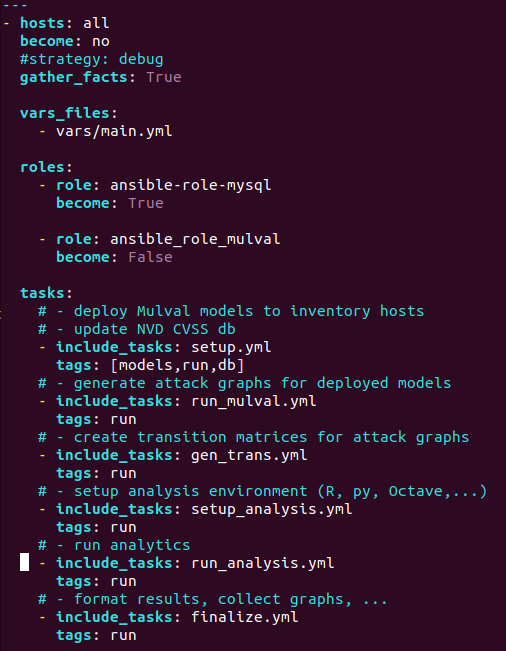
\includegraphics[width=.5\linewidth]{content/figs/deploy_infra/play.png}
% \caption{CSAF playbook}
% \label{fig:play}
% \end{figure} 

\begin{minipage}{\linewidth}
\begin{lstlisting}[language=yaml, label={lst:playbook}, caption={Ansible CSAF play},captionpos=b, linewidth=.6\textwidth]
 ---
- hosts: all
  become: no
  #strategy: debug
  gather_facts: True
  vars_files:
    - vars/main.yml
  roles:
    - role: ansible-role-mysql # NVD CVSS DB
      become: True
    - role: ansible-role-mulval # setup MulVal, XSB, etc
      become: False
  tasks:
    - include_tasks: setup.yml  # deploy models update NVD db
      tags: [models,run, db]
    - include_tasks: run.yml # generate attack graphs
      tags: [run, cleanup]
\end{lstlisting}
\end{minipage}

When preparing the target system, a directory containing the MulVal models to analyze is expected. These models are copied to the target system in individual directories as shown in Listing \ref{lst:model_dirs} since we can't control the output file names chosen by MulVal without modifying the distribution. 

\begin{minipage}{\linewidth}
\begin{lstlisting}[language=yaml, label={lst:model_dirs}, caption={MulVal distinct run dirs},captionpos=b, linewidth=.6\textwidth]
- name: copy models to remote in individual directories (mulval output is noisy)
  copy:
    src:  "{{item.path | relpath('{{mulval_models_src}}')}}"
    dest:  "{{mulval_models_dir}}/{{(item.path|basename|splitext)[0]}}"
  with_items: "{{find_results.files}}"
  tags: [models,run]
\end{lstlisting}
\end{minipage}

MulVal supports a single custom interaction rules file being passed as a runtime argument. To allow for a more customizable custom rules set, we allow for the rules defined per model or globally as shown in Listing \ref{lst:custom_rules}. Assuming the custom rules are defined in separate files in the \textit{mulval\_custom\_rules\_dir} directory, we can provide a list of rules for \textit{each} model we are testing, concatenate \textit{all} rules in the directory for every test, or omit custom rules for the test altogether.

\begin{minipage}{\linewidth}
\begin{lstlisting}[language=yaml, label={lst:custom_rules}, caption={MulVal custom rule strategies},captionpos=b, linewidth=.6\textwidth]
- name:  run mulval (all rules)
  shell: bash -lc "{{mulval_home}}/utils/graph_gen.sh {{ item.path|basename }} -p -v -a {{mulval_custom_rules_dir}}/custom_rules.P "
  args:
    chdir: "{{(item.path|dirname)}}"
  with_items: " {{ find_results.files }} "
  tags: run
  when: mulval_custom_rules_strategy == 'all'

- name:  run mulval (each rule)
  shell: bash -lc "{{mulval_home}}/utils/graph_gen.sh {{ item.path|basename }} -p -v -a {{mulval_custom_rules_dir}}/{{ item.path|basename }}.rules  "
  args:
    chdir: "{{(item.path|dirname)}}"
  with_items: " {{ find_results.files }} "
  tags: run
  when: mulval_custom_rules_strategy == 'each'

- name:  run mulval (no rules)
  shell: bash -lc "{{mulval_home}}/utils/graph_gen.sh {{ item.path|basename }} -p -v"
  args:
    chdir: "{{(item.path|dirname)}}"
  with_items: " {{ find_results.files }} "
  tags: run
  when: mulval_custom_rules_strategy == 'none'

\end{lstlisting}
\end{minipage}

After the CSAF framework has completed processing a set of models, results are collected by simply transferring them to the desired location as shown in Listing \ref{lst:collect_results}. Adding enhanced reporting and alerting capabilities as new results arrive can be achieved using a variety of monitoring tools (eg., inotify, db triggers, fluentd) depending on the destination.

\begin{minipage}{\linewidth}
\begin{lstlisting}[language=yaml, label={lst:collect_results}, caption={Collect Results},captionpos=b, linewidth=.6\textwidth]
- name: fetch results (get them all)
  synchronize:
   mode: pull
   src: "{{mulval_results_dir}}"
   dest: "{{mulval_output_dir}}"
   #with_items: "{{ find_results.files}}"
  tags: [run,collect]
\end{lstlisting}
\end{minipage}